% !TEX encoding = UTF-8 Unicode

\documentclass[twocolumn,10pt,a4j]{jsarticle}
\usepackage{kougai}

\title{積み上げ型教科の理解を促進させる
教育モデルの提案}
\author{1532009 阿部 希駿  指導教員 須田 宇宙 准教授}
\date{}

\begin{document}

\maketitle

\section{はじめに}

%背景
中学,高校で学習する科目の中で数学と英語は苦手になりやすいと言われている\cite{1}.この2科目の共通点として「積み上げ型教科」である点が挙げられる.積み上げ型教科とは学習した単元を前提知識として他の単元の学習を行う教科で,本研究では前提知識となる単元を「前提単元」,前提知識を用いて学習を行う単元を「主単元」と称する.積み上げ型教科では前提単元の具体例などのイメージをしづらいことが理解の妨げになっていると考える.
%問題点

そこで「主単元が具体例のわかりやすい単元であるとき,主単元の概要をあらかじめ学習することで,前提単元の理解を促進することができる」という仮説を立てた.
本研究では,学生を対象に講義にて実験を行い,この仮説を証明することを目的とする.



\section{実験の構想}

本研究では2018年後期に開講される情報数学応用の講義履修者を対象に対照実験を行う.
図\ref{fig:time}に示す順で1週目と2週目に講義を行い,3週目に小テストを行う.

\begin{figure}[H]
\centering
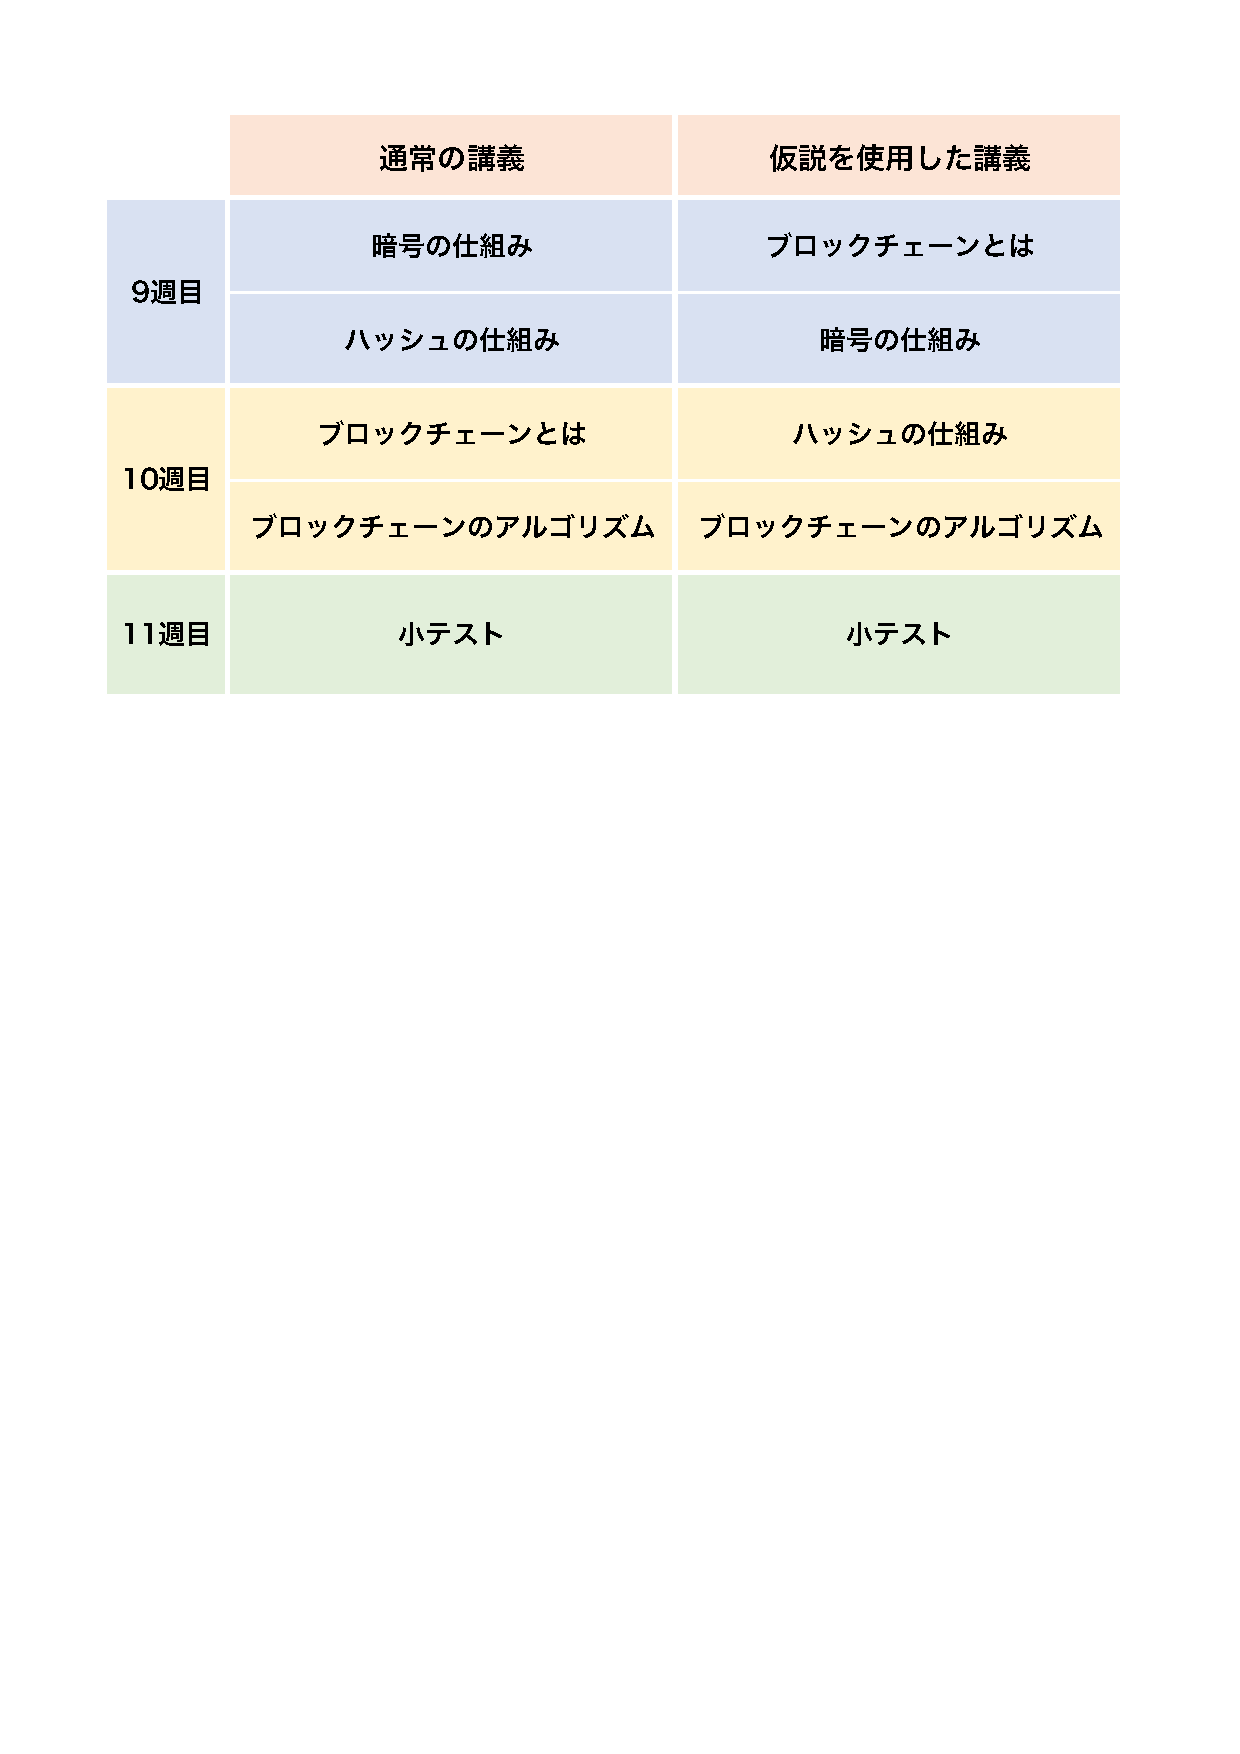
\includegraphics[mediaboxonly=/CropBox,width=9cm]{timeline.pdf}
\caption{実験で行う授業の流れ}
\label{fig:time}
\end{figure}


小テストでは以下の3項目の問題とアンケートを用意する.
\begin{enumerate}
\renewcommand {\labelenumi}{(\arabic{enumi})}
\item 暗号の仕組み
\item ハッシュと暗号の違い
\item ブロックチェーンの仕組み
\end{enumerate}

アンケートでは講義を受ける以前にブロックチェーンの仕組みについての知識の有無,「暗号」「ハッシュ」「ブロックチェーン」それぞれの講義内容がわかりやすかったかについて尋ねた.
「暗号の仕組み」と「ハッシュと暗号の仕組み」を前提単元,「ブロックチェーンの仕組み」を主単元とし,結果の分析は分けて行う.
2クラスの元の学力の影響を考え,中間試験と小テストの平均点の差を調べた.
そこで分析対象を中間試験の受験者かつブロックチェーンを講義前に学習していない学生とした.


\section{結果と考察}

小テストの結果,2クラスの点数に差は見られなかった.図\ref{fig:total}では合計点の得点分布を示す.

\begin{figure}[H]
\centering
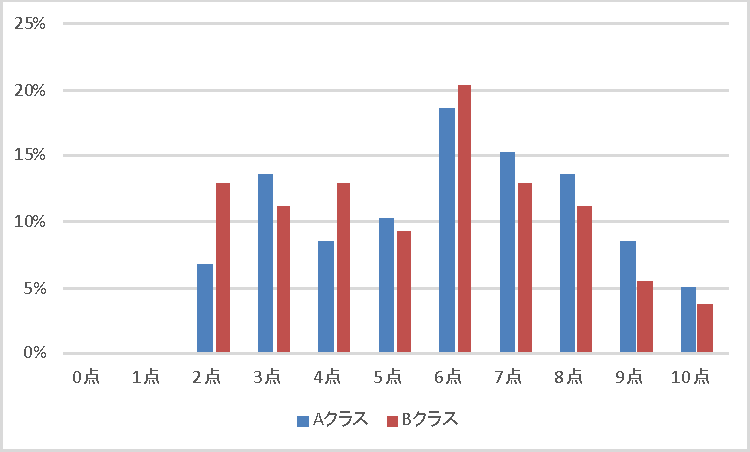
\includegraphics[width=8cm]{total.pdf}
\caption{小テストの合計点の得点分布}
\label{fig:total}
\end{figure}

仮説が証明できなかった原因を以下のように考察した.
\begin{itemize}
\item 仮説が間違えている.
\item アンケート結果より主単元よりも前提単元の方がわかりやすい内容であった.そのため具体例がわかりやすい単元が主単元となっておらず,主単元の選定が不適切であった.
\item 中間試験との点数の差を求めたが,中間試験の点数と小テストの点数には相関が見られなかったことから,講義以外のテスト勉強などの影響を多く受けた可能性があり,講義においての理解度が測れなかった.
小テストを行う事前予告をした上で,期間を空けたために,テスト勉強を行った学生の人数の差が大きかった可能性があり,講義のみでの理解度を測ることができなかった.
\item 「暗号・ハッシュ」と「ブロックチェーン」の平均点に大きく差が見られたことから問題の難易度に差があった.講義スケジュールの関係で1週目と2週目の間に休講日があり,前半にブロックチェーンの概要を学習したクラスの得点が下がった.
\end{itemize}

\section{おわりに}
本研究では積み上げ型教科の理解度を上げる仮説を立て,実験を行なった.今回の実験では仮説が正しいと証明することができなかったが,実験の改善点が見つかったため,今後はさらなる実験を行い検証することが望まれる.

\begin{thebibliography}{99}
\bibitem{1}
ベネッセ教育情報サイト:“教科学習が不得意と感じている高校生が9割!そのほとんどが英語と数学に偏るのにはある理由が”, \url{https://www.benesse.jp/kyouiku/201603/20160329-3.html}, (参照 2018-8-14)
\end{thebibliography}

\end{document}